%\documentclass{svjour3}                     % onecolumn (standard format)
%\documentclass[smallcondensed]{svjour3}     % onecolumn (ditto)
\documentclass[smallextended]{svjour3}       % onecolumn (second format)
%\documentclass[twocolumn]{svjour3}          % twocolumn
%
\smartqed  % flush right qed marks, e.g. at end of proof
%
\usepackage{array}
\usepackage{comment}
\usepackage{supertabular}
\usepackage{longtable}
\usepackage{booktabs}
\usepackage{multirow}
\usepackage{color}
\usepackage{tabulary}
\usepackage{CJKutf8}
\usepackage{graphicx}
\usepackage{natbib}
%\usepackage{amsmath}
%\usepackage{amssymb}
%\usepackage{amsthm}
\usepackage{algorithm}
\usepackage[noend]{algpseudocode}
\usepackage[small]{caption}
\usepackage{ulem}

%
% \usepackage{mathptmx}      % use Times fonts if available on your TeX system
%
% insert here the call for the packages your document requires
%\usepackage{latexsym}
% etc.
%
% please place your own definitions here and don't use \def but
% \newcommand{}{}
%
% Insert the name of "your journal" with
% \journalname{myjournal}
%
\begin{document}

\title{Automatic Discovery of Adverse Reactions through Chinese Social Media\thanks{*The authors contributed equally to this work.      **Corresponding authors}
%\thanks{Grants or other notes
%about the article that should go on the front page should be
%placed here. General acknowledgments should be placed at the end of the article.}
}
%\subtitle{Do you have a subtitle?\\ If so, write it here}

%\titlerunning{Short form of title}        % if too long for running head

\author{Mengxue Zhang$^{*}$\and
        Meizhuo Zhang$^{*}$\and
        Chen Ge\and
        Quanyang Liu\and
        Jiemin Wang\and
        Jia Wei$^{**}$\and
        Kenny Q. Zhu$^{**}$ %etc.
}

%\authorrunning{Short form of author list} % if too long for running head
\authorrunning{Mengxue Zhang et al.} % if too long for running head

\institute{Kenny Q. Zhu \at
              Dept. CSE, Shanghai Jiao Tong University, 800 Dongchuan Road, Shanghai 200240, China \\
              \email{kzhu@cs.sjtu.edu.cn}           %  \\
%             \emph{Present address:} of F. Author  %  if needed
           \and
           Jia Wei \at
              R\&D Information, AstraZeneca, 199 Liangjing Road, Pudong, Shanghai, 201203, China \\
              \email{Jenny.Wei@astrazeneca.com}
}

\date{Received: date / Accepted: date}
% The correct dates will be entered by the editor


\maketitle
%Please provide an abstract of 150 to 250 words. The abstract should not contain any undefined abbreviations or unspecified references.
\begin{abstract}
Despite tremendous efforts made before the release of every drug, some adverse drug reactions (ADRs) may go undetected and thus, cause harm to both the users and to the pharmaceutical companies. One plausible venue to collect evidence of such ADRs is online social media, where patients and doctors discuss medical conditions and their treatments. There is substantial previous research on ADRs extraction from English online forums. However, very limited research was done on Chinese data. In this paper, we try to use the posts from two popular Chinese social media as the original dataset. We propose a semi-supervised learning framework that detects mentions of medications and colloquial ADR terms and extracts lexicon-syntactic features from natural language text to recognize positive associations between drug use and ADRs. The key contribution is an automatic label generation algorithm, which requires very little manual annotation. This bootstrapping algorithm could also be further applied on English data. The research results indicate that our algorithm outperforms the hidden Markov model(HMM) and conditional random fields(CRF). With this approach, we discovered a large number of side effects for a variety of popular medicines in real world scenarios.
%Please provide 4 to 6 keywords which can be used for indexing purposes.
\keywords{adverse drug reaction \and Chinese social media \and natural language processing}
% \PACS{PACS code1 \and PACS code2 \and more}
% \subclass{MSC code1 \and MSC code2 \and more}
\end{abstract}
\begin{CJK}{UTF8}{gbsn}
\section{Introduction}
\label{intro}
Determination of adverse drug reactions (ADR) is an important part of pharmaceutical research and drug development. Pre-marketing clinical trials are limited by the number of participants, the length of the study and the underlying economic burden for both the pharmaceutical companies and the patients. Several recent researches try to predict the potential ADR of drug by using the drug chemical structures, protein targets or therapeutic indications during the drug development cycle\citep{scheiber2009mapping, xie2009drug, yamanishi2012drug, wang2014exploring, xiao2017adverse}. Some of the new adverse reactions to a drug are learned only when the drug is used in a wide spectrum of patients, with varied ethnicity, underlying diseases and a range of concomitant medication, in a post-launch setting. Furthermore, some reactions take a long time to develop a process which goes well beyond the pre-marketing development cycles of the drugs. For example, Vioxx, developed by Merck \& Co, was approved by the FDA in May 1999 as a nonsteroidal anti-inflammatory drug to treat osteoarthritis, acute pain and dysmenorrhea. However, other Merck \& Co sponsored studies, which were concluded or commenced after the drug was launched, indicated that it was associated with elevated risk of cardiovascular complications \citep{bombardier2000comparison,bresalier2005cardiovascular}. In September of 2004, Merck withdrew Vioxx from the market because of concerns about increased risk of heart attack and stroke associated with long-term, high-dosage use. An FDA study estimated that Vioxx could have caused up to 140, 000 cases of serious heart disease in the US since 1999 \citep{graham2005risk}.  Regulatory authorities and pharmaceutical companies make tremendous effort in avoiding such incidences by conducting post-launch Phase IV clinical trials. In the United States, drug companies spend up to \$12,000 per patient in Phase IV clinical trials, with an average of \$5,856 \footnote{https://www.cuttingedgeinfo.com/2011/us-phase-iv-budgets/}. Conducting such studies in an ``\textit{in silico}'' fashion, i.e., collecting ADRs from pre-existing data sources, has become a valid complement, if not an attractive alternative, to costly Phase IV studies.

Recent years saw a growing research interest in mining adverse drug reactions from various data sources. Data sources can be divided into structured data and unstructured text data, and the approaches differ. Structured data primarily includes official adverse event reports collected by health authorities~\citep{harpaz2010statistical,harpaz2012novel,hahn2012mining,gurulingappa2013automatic} such as
FDA. These reports are relatively easy to process due to their strict conformance to the adverse event reporting standards. However, the quantity of such reports is limited due to the complex procedure of submitting reports and patients' unawareness of spontaneous reporting systems. Unstructured data so far includes biomedical literature, clinical notes or medical records, and online health discussions. These data sources pose more processing challenges because signals are embedded in natural language, which is inherently ambiguous and noisy. Biomedical literatures such as scientific papers are comparatively easier to mine \citep{wang2011drug,yang2012automatic} since the medication and adverse reaction are referred to by their formal names. However, the information therein is not up-to-date and is sometimes biased. Clinical resources were targeted using various methods, such as text mining for identifying ADRs from medicine uses \citep{warrer2012using}, rule-based methods to extract side effects from clinical narratives \citep{sohn2011drug} and retrospective medication orders along with inpatient laboratory results to identify ADRs \citep{liu2013azdrugminer}. Privacy concerns and access restrictions are the biggest obstacles for its wide adoption. Compared to the above data sources, online social media, especially health discussion forums, provide the most comprehensive and timely information about medication use experiences. The large volume, colloquial use of natural language, spelling and grammatical errors are some of the major challenges in mining ADRs from such data sources. 

Existing methods for social media text mining can be categorized into lexicon-based methods, statistical methods, rule-based method, advanced NLP and neural network. Most prior studies \citep{leaman2010towards,yang2012detecting,benton2011identifying,wu2013exploiting,yates2013ADRTrace,liu2014identifying,jiang2013discovering,freifeld2014digital,yeleswarapu2014pipeline} focused on expanding lexicons to find ADRs in text. In these lexicon-based methods, due to the novel adverse reaction phrases on websites, they could not recognize non-regular ADRs that are not contained in the lexicon. Besides, they suffer from poor approximate string matching caused by misspelled words. Some researchers instead utilized statistical \citep{li2011medical,wu2012early,liu2013azdrugminer}, rule (pattern) based methods \citep{nikfarjam2011pattern,benton2011identifying,karimi2011drug,yang2012detecting}; When it comes to NLP techniques, common approaches used Support Vector Machine(SVM) and Conditional Random Field(CRF) to detect ADR from social media\citep{sharif2014detecting,sarker2015portable,jonnagaddala2016binary,nikfarjam2015pharmacovigilance}. They always consider different features such as N-grams, POS tags, negation, sentiment word, polarity and etc. These methods could offer a reasonable accuracy, however they are built with supervised training and require large volume of data during the learning process which requires a tremendous amount of manual effort. Various architectures of neural network have also been researched for the detection of ADRs. People have tried convolutional neural network\citep{lee2017adverse}, recurrent neural network\citep{cocos2017deep} or combine them together\citep{huynh2016adverse}. Moreover, attention mechanism and CRF are sometimes added into the architecture to improve the performance of system\citep{pandey2017improving}. 

Although there is substantial previous research on ADRs extraction from English online forums, very limited research was done on Chinese data. To the best of our knowledge, this paper is the first attempt to mine ADRs from two popular Chinese social media sites, namely Xunyiwenyao \footnote{http://club.xywy.com/} and 
Haodaifu \footnote{http://www.haodf.com/}. Xunyiwenyao and Haodaifu are both online public forums for health-related discussions. 
We have also attempted to use the data from Weibo\footnote{http://weibo.com} which is a Chinese microblogging website. However, very few Weibo messages contain a drug and an ADR at the same time, and most of the messages are noisy. 
For example, among all the messages we crawled from Weibo, 7734 messages 
mentioned Betaloc, but only 1323 of these also contain an ADR. 
After viewing these messages, only 36\% of them are really experience reports 
from the patients who have taken that medicine.
In consequence, we only use the the data from ``Xunyiwenyao'' and ``Haodaifu'' 
in this paper to discover the potential ADRs.

Herein, we propose a semi-supervised learning framework requiring very little manual annotations for mining ADRs from Chinese social media. As an alternative to the methods described above, we build a list of commonly misspelled drug names and extend the customized lexicon with colloquial words and adjective modifiers, in order to address the problem of irregular ADR terms and typos. We also focus on distinguishing between indications and ADRs by training a binary classifier, using the SVM model. To train the classifier, we introduce an automatic labeling algorithm to generate large amount of training data.

\section{Methods}
\label{methods}
% For one-column wide figures use
\begin{figure}
	% Use the relevant command to insert your figure file.
	% For example, with the graphicx package use
	\centering
	\includegraphics[width=0.6\columnwidth]{Fig1.eps}
%	\resizebox{0.8\hsize}{!}{\includegraphics*{firstFig1-01.eps}}
%	\includegraphics{firstFig1-01.eps}
	% figure caption is below the figure
	\caption{System framework}
	\label{fig:1}       % Give a unique label
\end{figure}
%
Our framework (depicted in Fig.~\ref{fig:1}) is divided into four parts, namely constructing lexica, extracting candidate ADRs, classifying evidences and finally ranking the ADRs.

\subsection{Lexicon construction}
\label{subsec:2.1}
We need two lexicons, one for the names of medications of interest; the other for ADRs to be recognized from text.

\subsubsection{Lexicon of medication}
\label{subsubsec:2.1.1} 
We start with a list that contains common names and registered trade names of known drugs. 
On social media, drug names may be spelled with variation, either by similar characters or 
homophones. For example, a drug called “耐信(Nexium)”(nài xìn in Chinese phonetic alphabet)  
may be misspelled as “奈信”(nài  xìn), “乃信”(nǎi xìn) and so on. To solve this problem, we expand each correct character in a drug name to several commonly misspelled characters in Chinese according to the Chinese phonetic alphabet. For example, “耐” is extended to “奈” or “乃”, while “信” is extended to “心”, “新” and so on. However, if “耐信” is transformed to “耐心”, which is a commonly used Chinese word, many irrelevant posts containing “耐心” maybe returned. Thus common Chinese words which are clearly not drug names are filtered out. After this kind of expansion, we obtain a total of 110779 different drug names for 79 drugs of interest. The list of all these 79 drugs of interest can be found in Appendix \ref{apx:drugs}.

% For tables use
\begin{table}
	% table caption is above the table
	\centering
	\caption{ADRs lexicon}
	\label{tab:1}       % Give a unique label
	% For LaTeX tables use
	%	\begin{tabular}{llll}
	\begin{tabular}{p{2cm}p{2cm}p{2cm}p{2cm}}
		%	\begin{tabular}{0.4\textwidth}{llll}
		\hline\noalign{\smallskip}
		5’-核苷酸酶下降(5'-nucleotidase decline)&各种肝功能分析(Variety of liver function)&肝胆系统检查(Hepatobiliary system check)&各类检查(Various types of inspection) \\
		\noalign{\smallskip}\hline
		5’-核苷酸酶增加(5'-nucleotidase increase)&各种肝功能分析(Variety of liver function)&肝胆系统检查(Hepatobiliary system check)&各类检查(Various types of inspection)\\
		\noalign{\smallskip}\hline
		A型肝炎(Hepatitis A)&各种肝脏病毒感染(Various liver virus infection)&肝脏及肝胆类疾病(Liver and hepatobiliary diseases)&肝胆系统疾病(Hepatobiliary system diseases)\\	
		\noalign{\smallskip}\hline
		BK病毒感染(BK virus infection)&多瘤病毒感染(Polyomavirus infection)&传染性病毒感染(Contagious viral infection)&感染及侵染类疾病(Infection and infection diseases)
		\\
		\noalign{\smallskip}\hline
	\end{tabular}
\end{table}

\subsubsection{Basic ADR lexicon}
\label{subsubsec:2.1.2} 
The basic ADR lexicon comes from four sources: NCI Common Terminology Criteria for Adverse Events (CTCAE) \citep{trotti2003ctcae}, Sougou Pinyin ADRs lexicon\footnote{Sogou Pinyin is a Chinese input method, and there are many available lexicons, one of which is the 
ADRs lexicon: http://pinyin.sogou.com/dict/detail/index/644 .}, 
MedDRA(The Medical Dictionary for Regulatory Activities) \citep{brown1999the} and 
the ADR database by Ye et al \citep{ye2014construction}. CTCAE contains formal terms of 
the ADRs used for adverse event reporting to regulatory agencies. Sougou ADRs is utilized particularly for colloquial terms. Here are some examples: “听力降低”(poor hearing), “焦急不安”(anxious), “健忘”(forgetful), “头发稀疏”(hair thinning). Both CTCAE and Sougou ADRs are available in Chinese. The ADRs database covers more than 6000 ADRs in English. It was translated into Chinese by Google Translate\footnote{https://translate.google.com/}. In addition, classification of these terms is very important. Because some words have the same or similar meaning, their results can be merged in the following analysis steps. For example, “体重减少” (loss of weight) is the same as “体重下降” (drop in weight). If we classify both words in the same category, their result can be directly added and we get one total result for later discussion. Finally, based on MedDRA’s category, we classify all the words into structured lexicon which has four levels. The lowest level contains ADR words from the three data sources. The three upper levels are custom categories in MedDRA. In Table~\ref{tab:1}, the first column in the left is the fourth level and the next three columns are the upper levels in MedDRA.

\subsubsection{Extended ADR lexicon}
\label{subsubsec:2.1.3} 
To improve the ability to match colloquial terms in online discussion, we further expand our basic ADR lexicon by adding variations of the terms. For example, when a person has a headache, he or she may say “头痛(headache)” or “头有点痛(got a little headache)”, the latter of which is a slight variation with a degree modifier between an organ name and symptom word such as “痛” (pain), and is added to our extended lexicon.

There is a variety of such degree modifiers. We adopt a data-driven approach to mine such degree modifiers by pattern-matching an organ name, up to 5 characters and a symptom word, for example “头(head)XXXXX 痛(pain)”, from online discussion corpus. The algorithm to extend ADR lexicon is presented briefly as Algorithm \ref{algo:extlex}.

\begin{algorithm}
\caption{Extending ADR lexicon}
\label{algo:extlex}
\begin{algorithmic}[1]
\State{//Construct regular expression patterns}
\For {each term in basic ADRs}
	\If {term contains organ} 
		\State{construct a regular pattern}
	\EndIf
\EndFor
\State{//Discover degree words}
\For{each line in all data}
	\If{line match a pattern then}
		\State{count one for this word} 
	\EndIf
\EndFor
\State{//Extend lexicon} 
\For{each term in lexicon}
	\If{term contains organ} 
		\For{each word in words list} 
			\State{insert word into term to generate a new term} 
		\EndFor
	\EndIf
\EndFor
\end{algorithmic}
\end{algorithm}

\subsection{Data sources and data preparation}
\label{subsec:2.2}
This section describes two Chinese social media and how we extract evidences of ADRs for drugs from them.

\begin{figure}\sidecaption
\centering
	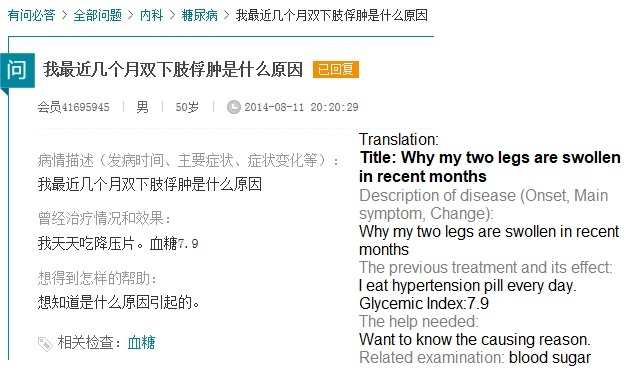
\includegraphics[width=0.9\columnwidth]{Fig2.jpg}
%	\resizebox{0.3\hsize}{!}{\includegraphics*{xywyExample.jpg}}
	\caption{Question posted on Xunyiwenyao website}
%	\definecolor{defGrey}{RGB}{128,138,135}
%	 Translation:\\
%		\textbf{Title: Why my two legs are swollen in recent months} \\
%		\textcolor{defGrey}{Description of disease (Onset, Main symptom, Change):}\\
%		Why my two legs are swollen in recent months\\
%		\textcolor{defGrey}{The previous treatment and its effect:}\\
%		I eat hypertension pill every day. Glycemic Index:7.9\\
%		\textcolor{defGrey}{The help needed:}\\
%		Want to know the causing reason.\\
%		\textcolor{defGrey}{Related examination:} blood sugar
	%	\\

	\label{fig:2}	
\end{figure}

\subsubsection{Chinese social media}
\label{subsubsec:2.2.1} 
Xunyiwenyao was established in 2004. By 2014, it has over 80,000,000 registered accounts, 
over 20,000,000 daily independent, and is ranked first in the medical and health service 
industry. The forum contains 14 categories and 64,050 discussion threads on average, 
every day. Each discussion thread starts with a patient’s question, which is followed by 
responses from multiple doctors or other patients (see Fig.~\ref{fig:2}).

Haodaifu was launched in 2006. Its physician-patient interactive forum is 
the largest in China, with over 501,000 registered healthcare professionals. 
It contains 29 categories and 18,632,602 discussion threads until now. 
The format of the discussion is similar to Xunyiwenyao.

\subsubsection{Extraction of evidences}
\label{subsubsec:2.2.3} 
First, we preprocess all the user posts from three websites. If one post contains a drug name of interest, this post is considered as an ``effective'' target. All sentences in ``effective'' posts are segmented by ICTCLAS \citep{zhang2003hhmm}, a Chinese word segmentation tool.

With the ADR lexicon, we can detect candidate ADR terms from the effective posts. However, when a drug name $X$ is mentioned in a post, the user may not actually have taken that drug. Similarly, when an ADR term is mentioned, the user may not actually have the symptom, or the symptom may not be the result of taking $X$. Therefore, given a pair of a drug name and an ADR, we need to determine whether the ADR is truly the consequence of taking the drug, given the context of the pair in the post. Because of that a drug-ADR pair that is too far away from each other in the text is not reliable, the context is defined as one or more consecutive sentences where the distance between drug and ADR is less than 55 Chinese words (including punctuations but excluding spaces). We ensure that each context contains one drug-ADR pair.

We define a context as a positive evidence if the candidate ADR in the context is a real ADR, while the other cases belong to the negative sentence. The following are two contexts showing a positive evidence and a negative evidence:

\begin{itemize}
	\item 服用\uline{易瑞沙}后\uline{头痛},眼睛复视,模糊 (After taking \uline{Iressa}, had a \uline{headache}, eye diplopia and blurred vision)
	\item 吃的是\uline{奥美拉唑},克拉霉素,阿莫西林,吗丁啉等药,\uline{咳嗽}有所减少 (After taking \uline{Omeprazole}, Clarithromycin, Amoxicillin, Domperidone and other drugs, \uline{cough} lessened) 
\end{itemize}

\subsubsection{Data set}
\label{subsubsec:2.2.4} 

\begin{table}
\centering
	% table caption is above the table
	\caption{Category of drugs studied}
	\label{tab:2}       % Give a unique label
	% For LaTeX tables use
	\begin{tabular}{llll}
%	\begin{tabular}{p{2cm}p{2cm}p{2cm}p{2cm}}
		%	\begin{tabular}{0.4\textwidth}{llll}
		\hline\noalign{\smallskip}
		Category & Number of drugs & Diseases & Number of drugs \\
		\noalign{\smallskip}\hline
		Hypertension & 29 & Hyperacidity & 2 \\
		Diabetes & 18 & Lung cancer & 1 \\
		Asthma & 15 & Rhinitis & 1 \\
		Statins & 9 & Schizophrenia & 1 \\
		Breast cancer & 1 & Acute coronary syndrome & 1 \\
		Anesthesia & 1 \\
		\noalign{\smallskip}\hline
	\end{tabular}
\end{table}


We have crawled user messages posted between January 2011 to April 2015 on Haodaifu and Xunyiwenyao. These messages mentioned 79 drugs, which treat 11 types of diseases. Table~\ref{tab:2} summarizes the diseases and the number of corresponding drugs. In total, 456,753 posts were crawled.

After preprocessing these posts, we obtain 302,180 sentences where a drug-ADR pair is revealed. We first manually label 1200 sentences which contains 600 positive evidences and 600 negative evidences. Then we divide them into training set, tuning set and test set. Finally, we get a training set with 300 positive evidences and 300 negative evidences, a tuning set with 200 positive evidences and 200 negative evidences and a test set with 100 positive evidences and 100 negative evidences.

\subsection{Evidence Classifier}
\label{subsec:2.3}
Given a drug name and a medical condition, identified by the extended lexicon, as well as their context in the original text, the problem of evidence classification is to determine whether the medical condition is actually an ADR resulting from the drug. Next we present a method to train such an evidence classifier. In particular, we show how to produce large amount of training data by automatic labeling.

\subsubsection{Building the training set}
\label{subsubsec:2.3.1} 
A supervised classifier requires labeled training data. However, manual labeling on user discussion posts can’t scale up because of the large amount of informal use of language and colloquial terms. Fortunately, information in the package insert of the drugs, e.g., the indications and the known side effects of the drug, can be used to automatically generate labeled data. 

Our first and simple idea is to regard a pair of drug and medical condition as true if the medical condition is listed as a side effect in the package insert of the drug. Conversely, we regard the pair as false if the medical condition is listed as an indication of the drug. All other pairs are discarded from labeled data set. However, this approach is not perfect. For example, “头晕(dizzyness)” is a known ADR for Betaloc, but sometimes in the real discussion it serves as an indication:

\begin{itemize}
	\item 突然感到\uline{头晕心慌},坐卧不安,去医院检查血压160.100 心电图心动过速160次,开了\uline{倍他乐克}(Suddenly I felt \uline{dizzy}, flustered, and restless, my blood pressure was at 160/100; tachycardia electrocardiogram was at 160 times. Consequently I was given \uline{Betaloc})
\end{itemize}

Similarly, “房颤(atrial fibrillation)” is an indication for Betaloc, but sometimes it is reported as if it’s a side effect:

\begin{itemize}
	\item 后根据医嘱,可达龙减至1/4片每天,加服\uline{倍他乐克}缓释片一片。一段时间后出现\uline{房颤}(According to the doctor’s advice, Cordarone was reduced to 1/4 tablets per day, plus one tablet of \uline{Betaloc}(slow release). \uline{Atrial fibrillation} occurred after a period of time)
\end{itemize}

Because the actual situation arising from patients’ experience may be more complicated than specified on the inserts, we adopt a semi-supervised approach instead. We first use the 
600 manually labeled data to train a simple SVM classifier and use it to predict for all 
the sentences in the corpus. The features used are discussed in 
Section \ref{subsubsec:2.3.2}. If the classifier predicts a sentence to be positive, 
and the medical condition is a known ADR for the drug according to the insert, 
we add this sentence into the new positive training set. If a sentence is predicted to be negative, and the condition in that sentence is a known indication of the drug, then we add this sentence into the negative training set. We exclude those sentences for which the 
prediction of classifier and content of the package insert are different. 
The new training set also contains our original 600 manual labeling data.

With little manual effort, we have now obtained a much larger set 
of positive and negative training data (called semi-supervised data) --- 
12,238 training instances in total. By manual validation, the accuracy of such 
automatic labeling is 82\%.

\subsubsection{Features extraction}
\label{subsubsec:2.3.2}
Our main evidence classifier extracts the following features (see Table\ref{tab:2.1}), after parsing the evidence sentences into dependency trees:

\begin{table}
	\centering
	\caption{Features that we extracted}
	\label{tab:2.1}       % Give a unique label
	% For LaTeX tables use
	%	\begin{tabular}{lllllll}
	\begin{tabular}{m{1.2cm}m{5cm}m{4cm}}
		\hline\noalign{\smallskip}
		Notation & Description & Examples \\
		\noalign{\smallskip}\hline\noalign{\smallskip}
		Feature 1 & Verbs before the drugs & “服用(take)” in “服用倍他乐克(take \textit{Betaloc})” \\
		Feature 2 & Verbs before the conditions & “感到(feel)” in “感到头晕(feel dizzy) \\
		Feature 3 & Verbs after the conditions & “好转(improved)” in “头疼好转(headache improved)” \\
		Feature 4 & Preposition, conjunction and noun of locality & “因为(because of)” in “因为头疼(because of headaches)” and “后(after)” in “服用倍他乐克后(after taking \textit{Betaloc})” \\
		Feature 5 & Punctuations that surround drugs and conditions & “,” and “。” in “吃完后,感到头疼。(feel headache after eating)” \\
		Feature 6 & The number of other drugs and other conditions between the drug and condition of interest & Both numbers are equaling to 1 in the sentence “服用信必可和舒利迭之后,感到头痛,身上有些地方还有荨麻疹(After taking \textit{Symbicort} and \textit{Seretide}, feel headache, there also appears urticaria in some places) if the drug and condition of interest is “信必可(Symbicort)” and “荨麻疹(urticaria)” \\
		Feature 7 & A boolean value that indicates whether condition appears in front of the drug or not & "true" in "因为哮喘,医生开了信必可(Because of asthma, the docter prescribed \textit{Symbicort})" and "false" for the sentence “用信必可来治疗哮喘(use \textit{Symbicort} to treat asthma)”\\
		\noalign{\smallskip}\hline
	\end{tabular}
\end{table}

\begin{comment}
\begin{enumerate}
	\item Verbs before the drugs, e.g. “服用(take)” in “服用倍他乐克(take \textit{Betaloc})”;
	\item Verbs before the conditions, e.g. “感到(feel)” in “感到头晕(feel dizzy)”;
	\item Verbs after the conditions, e.g. “好转(improved)” in “头疼好转(headache improved)”;
	\item Preposition, conjunction and noun of locality, e.g. “因为(because of)” in “因为头疼(because of headaches)” and “后(after)” in “服用倍他乐克后(after taking \textit{Betaloc})”;
	\item Punctuations that surround drugs and conditions;
	\item The number of other drugs and other conditions between the drug and condition of interest;
	\item A boolean value that indicates whether condition appears in front of the drug or not.
\end{enumerate}
\end{comment}
%The verbs are hard to extract without parsing the sentences. They often occur along with modifiers in the Chinese language. For example, “头疼好转(headaches improved)” would often be expressed as “头疼稍微好转(headaches improved a little bit)”, and with the dependency tree we can extract “好转(improved)” from it easily. 
The set of features described in Table\ref{tab:2.1} are used in both the initial and the final classifier. However, with more training data, the final classifier can better distinguish unseen tokens.
It’s worth noting that all these seven features are independent of the name of the drug 
and the ADR.

\subsubsection{Automatic labeling by bootstrapping}
\label{subsubsec:2.3.3}
We choose SVM as our primary classifier, because our feature vectors are high-dimensional (many different words). The overall process of our method is indicated in Algorithm.\ref{algo:bootstrap}.

\begin{algorithm}
	\caption{Automatic labeling by bootstrapping}
	\label{algo:bootstrap}
	\begin{algorithmic}[1]
		\State{Manually label small amount of seed data \textit{S}}
		\State{Train an initial SVM classifier M from \textit{S}}
		\State{Calculate F1-score of this SVM classifier based on the test data set}
		\Repeat
		%\While {F1-score not converge}
			\State{//Use \textit{M} to classify all the sentences and enlarge our training set with the help of packet inserts}
			\For {each sentence in corpus}
				\If {\textit{M} predicts this sentence to be positive \&\& the medication condition is a known ADR for the drug according to the packet insert}
					\State{Add this sentence to the positive training set}
				\ElsIf {M predicts this sentence to be negative \&\& the medication condition is a known indication of the drug according to the packet insert}
					\State{Add this sentence to the negative training set}
					\Else {\space keep this sentence in the corpus}
				\EndIf
			\EndFor
			\State{//update the SVM classifier}
			\State{Use the new training set to train a new SVM classifier and update \textit{M}}
			\State{Calculate F1-score of the updated classifier \textit{M} based on the test data set}
		%\EndWhile
		\Until {F1-score converge}
	\end{algorithmic}
\end{algorithm}


The above algorithm uses the package inserts and the initial classifier $M’$ to generate more training data. One interesting thought is to use that newly obtained classifier $M$ to label even more training data, and thus build a newer classifier. This process can go on iteratively until no more new training data is obtained. We will show the results of this in Section 3. The training data obtained at the final iteration is called semi-supervised data and will be used to train our SVM classifier and the other baseline classifiers (see Section~\ref{subsec:2.4}).

\subsection{Baseline classifier techniques}
\label{subsec:2.4}
\subsubsection{Pattern-based method}
\label{subsubsec:2.4.1}
Beside the above semi-supervised learning method, we have also tried a 
intuitive pattern-based classifier as a baseline. We extract preposition, 
conjunction and noun of locality from sentences as patterns from training data generated 
by package inserts. Each pattern has a weight, which is its frequency of occurrence; 
a negative pattern extracted from negative examples will have a negative weight. 
For example, below are two patterns we extracted and their weight:

\begin{itemize}
	\item drug ... 后 ... adr ... \quad 20
	\item adr ... 后 ... drug ... \quad -3
\end{itemize}

For a new sentence that can be matched to several patterns, the score is the sum of these patterns. Then a classifier is built based on the score: if the score is greater than 0, it’s positive; otherwise negative.

\subsubsection{HMM-based classifier}
\label{subsubsec:2.4.2}
We train a HMM classifier \citep{sampathkumar2014mining}. Particularly, comparing to original HMM paper where the sentences to be classified may not contain a drug-ADR pair, our task is more challenging because we firstly ensure a drug-ADR pair in all sentences and then make the classification.
We train two HMM classifiers in all. One classifier is only trained with 600 manually-labeled data and another classifier is trained with the semi-supervised data by using the package insert.

\subsubsection{CRF-based classifier}
\label{subsubsec:2.4.3}
We train a CRF-based classifier \citep{nikfarjam2015pharmacovigilance}. We also use two kind of data to train the two CRF-based classifiers: one with 600 manually-labeled data and another with semi-supervised data.
\\

Both the HMM and CRF classifiers were slightly modified to adapt to the Chinese input. For example we use ICTCLAS to segment and POS to tag the input sentences. 

\subsection{Ranking}
\label{subsec:2.5}
For each drug, there are many candidate ADRs. We are interested in those of high confidence. 
One way of ranking the ADRs of a drug is by the number of its appearances in positive 
evidence posts. This doesn’t work well because, most discussions about a drug involves the 
indications of the drug. For example, discussion about \textit{Betaloc} would naturally 
include a lot of occurrences of the term ``hypertension'' and the absolute number of such 
mentions is very large. Although our classifier can give a high accuracy, 
a number of sentences which contains ``hypertension'' as ADR are incorrectly predicted to 
be positive. Consequently, ``hypertension'' would be ranked highly as an ADR of 
\textit{Betaloc}. To solve this problem, we rank the ADRs according to the frequency of 
the positive evidences minus that of the negative evidences. This approach effectively 
lowers the rankings of the indications of a drug, but promotes real ADRs.

\section{Results}
\label{results}
We divide our evaluation into six parts. Firstly, we run the automatically labeling algorithm iteratively and show the change of the performance. Secondly, we will examine the importance of different features in the SVM classifier. Thirdly, we compare the accuracy of our final classifier with other several baseline classifiers (HMM, CRF and pattern-based), the difference caused by the difference training set will also be shown. Fourthly, we evaluate the effect of enlarging the drug and ADR lexica. Finally, we evaluate the accuracy of discovered ADRs with the help of drug package inserts, and show the top-ten discovered ADRs of several drugs, as verification and supplement for the known ADRs in the package inserts.

\subsection{Impact of the iteration}
\label{subsec:3.1}
\begin{figure}
\centering
	\includegraphics[width=0.6\columnwidth]{Fig3.eps}
	\caption{F1-score, accuracy and training data size of the new SVM classifier at 
each iteration}
	\label{fig:3}       % Give a unique label
\end{figure}

Fig.~\ref{fig:3} shows the accuracies and F1-scores on the tuning set after each iteration, using the bootstrapping approach in Section~\ref{subsec:2.3}. The result at iteration 0 is obtained using only the manually labeled data. After each iteration, the training set will enlarge, however the speed of growth becomes slow in each iteration and drops to 0 at 15$^{th}$ iteration. By using the tuning set which contains 400 manually labeled data (200 positive + 200 negative) to calculate the f1-score and accuracy of our SVM classifier in each iteration, we observe quick convergence: the two values keep constant after 9$^{th}$ iteration. 

The biggest improvement of performance comes from the 0$^{th}$ iteration to the 
1$^{st}$ iteration since the most knowledge is acquired in the first round of 
bootstrapping. The gain in accuracy and f1-score saturates after a peak is reached at 
the 5$^{th}$ iteration. We therefore use the training data obtained at that time to 
train our final SVM classifier and other baseline classifiers.

\subsection{The effectiveness of classification features}
\label{subsec:3.2}

\begin{table}
	\centering
	\caption{The effectiveness of classification features}
	\label{tab:3}       % Give a unique label
	% For LaTeX tables use
%	\begin{tabular}{lllllll}
	\begin{tabular}{m{2.5cm}m{1.4cm}m{1.4cm}m{0.8cm}m{0.8cm}m{0.8cm}m{1cm}}
		\hline\noalign{\smallskip}
		SVM Features & positive pairs & negative pairs & R & P & F1 & accuracy \\
		\noalign{\smallskip}\hline\noalign{\smallskip}
		All & 184/200 & 148/200 & 0.92 & 0.78 & \textbf{0.844} & \textbf{0.830} \\
		without feature 1 & 175/200 & 152/200 & 0.875 & 0.785 & 0.827* & 0.818 \\
		without feature 2 & 184/200 & 147/200 & 0.92 & 0.776 & 0.842 & 0.828 \\
		without feature 3 & 175/200 & \textbf{153}/200 & 0.875 & \textbf{0.789} & 0.829* & 0.820 \\
		without feature 4 & \textbf{187}/200 & 144/200 & \textbf{0.935} & 0.770 & \textbf{0.844} & 0.828 \\
		without feature 5 & 169/200 & 131/200 & 0.845 & 0.710 & 0.772* & 0.750 \\
		without feature 6 & 180/200 & 141/200 & 0.900 & 0.753 & 0.820* & 0.803 \\
		without feature 7 & 173/200 & 146/200 & 0.865 & 0.762 & 0.810* & 0.798 \\
		\noalign{\smallskip}\hline
	\end{tabular}
\end{table}

To examine the contribution of each feature of our SVM classifier, we use the previous tuning set which contains 400 manually labeled sentences to performed ablation tests on the tuning set. The result is shown in Table~\ref{tab:3}. Compared with All features set, those significant changes (the difference of F1-score is more than 0.10) are marked with asterisks. Besides, the highest values in each column are highlighted in bold.

We find that each feature does the contribution for the performance of the classifier. Among all the features, feature 1, 3, 5, 6, 7 are the most important ones as F1-score decreases sigificantly without these features.

\subsection{Drug-ADR association}
\label{subsec:3.3}

\begin{table}
	\centering
	\caption{Performance of various classifier}
	\label{tab:4}       % Give a unique label
	% For LaTeX tables use
	%	\begin{tabular}{lllllll}
	\begin{tabular}{m{3cm}m{1.2cm}m{1.2cm}m{1.2cm}m{1.2cm}m{1.2cm}}
		\hline\noalign{\smallskip}
		Methods & positive pairs & negative pairs & Recall & Precision & F1-score \\
		\noalign{\smallskip}\hline\noalign{\smallskip}
		Manual labels (Pattern-based) & 24/100 & 97/100 & 0.24 & \textbf{0.889} & 0.378 \\
		Manual labels (HMM) & 62/100 & 85/100 & 0.62 & 0.805 & 0.700 \\
		Manual labels (CRF) & 86/100 & 75/100 & 0.86 & 0.775 & 0.815 \\
		Manual labels (SVM) & 68/100 & 87/100 & 0.68 & 0.840 & 0.751 \\
		Auto labels from inserts (Pattern-based) & 47/100 & 77/100 & 0.47 & 0.671 & 0.553 \\
		Auto labels from inserts (HMM) & 85/100 & 55/100 & 0.85 & 0.654 & 0.739 \\
		Auto labels from inserts (CRF) & 98/100 & 32/100 & \textbf{0.98} & 0.590 & 0.737 \\ 
		Auto labels from inserts (SVM) & 81/100 & 65/100 & 0.81 & 0.698 & 0.75 \\
		Semi-supervised labels (Pattern-based) & 76/100 & 89/100 & 0.76 & 0.874 & 0.813 \\
		Semi-supervised labels (HMM) & 87/100 & 54/100 & 0.87 & 0.654 & 0.747 \\
		Semi-supervised labels (CRF) & 98/100 & 34/100 & \textbf{0.98} & 0.598 & 0.742 \\
		Semi-supervised labels (SVM) & 86/100 & 79/100 & 0.86 & 0.804 & \textbf{0.831} \\	 
		\noalign{\smallskip}\hline
	\end{tabular}
\end{table}

According to the previous research, we use the training data obtained at the 5$^{th}$ iteration and all the features to train our SVM classifier. To make the comparison with several baseline classifiers, another 200 manually-labeled test data (100 positive + 100 negative), which are different from the previous tuning set, is chosen to check the performance of the various classifier. The result is shown in Table~\ref{tab:4}. There are three kinds of training data:

\begin{itemize}
	\item \textbf{Manual labels:} use the manually labeled training set with 300 positive instances and 300 negative instances
	\item \textbf{Auto labels from insert:} use the  training data that we obtained according to the package insert directly without help of the manually labeled data. If the symptom in the sentence is ADR according to the package insert, it will be added into positive training set. Inversely, if the symptom in the sentence is indication according to the package insert, it will be added into negative training set. 
	\item \textbf{Semi-supervised labels:} use the training data that we obtained after the 5$^{th}$ iteration.
\end{itemize}

The pattern-based classifier depends a lot on the size of the training data set. More training data could help it to recognize more patterns of a positive sentence. In consequence, the performance improves a lot when using semi-supervised labels.

The HMM-based classifier emphasizes on the structure of sentences. The performance improved if the structure in training set and testing set is standard. Therefore, when we use the manually-labeled data to train the HMM classifier, the small size of training data set results in a low precision. It can be also seen that the percentage of true positives is inversely correlated with the percentage of true negatives. This means a classifier is biased to produce either more positive labels or more negative labels. A good classifier, such as the one trained with the semi-supervised labels manages to strike a balance between the two biases and produce a better overall F1-score.

CRF-based classifier use the sequence labeling with word embedding cluster features, which reduces the effect of the training set’s size. However, this kind of classifier also depends on the grammatical form of a sentence. When training set enlarges, the structure of negative instances becomes various and do not have a regular form, which leads to a bad performance of the CRF classifier.

In short, both the HMM and CRF concentrate more on the information of the single word itself and its limited surrounding words. However, SVM focus on the features of the whole sentence.

The semi-supervised data, which is doubly verified by the primary SVM classifier and package inserts, may not have a very standard form (e.g., some sentences do not have the causal keyword but have a lot of noisy words between the ADR and its associated drug). For those user posts, which do not have a standard form, SVM performs clearly better because of its global view, and HMM doesn’t perform as well because it requires sentences in their standard form.

\subsection{Homophone transformation and extended ADR lexicon}
\label{subsec:3.4}

\begin{table}
	\centering
	\caption{Enlarging data set through homophone transform}
	\label{tab:5}       % Give a unique label
	% For LaTeX tables use
	%	\begin{tabular}{lllllll}
	\begin{tabular}{m{2cm}m{1.2cm}m{1.2cm}m{1.2cm}m{1.2cm}m{1.2cm}}
		\hline\noalign{\smallskip}
		& 倍他乐克 (Betaloc) & 耐信 (Nexium) & 拜唐苹 (Glucobay) & 氨茶碱 (Aminophylline) & All 79 drugs \\
		\noalign{\smallskip}\hline\noalign{\smallskip}
		official name & 24073 & 6521 & 530 & 7493 & 158695 \\
		homophone & 13177 & 6369 & 1611 & 2388 & 143485 \\
		total & 37250 & 12890 & 2141 & 9881 & 302180 \\
		\%increase & 35.4\% & 49.4\% & 75.2\% & 24.2\% & 47.5\% \\ 
		\noalign{\smallskip}\hline
	\end{tabular}
\end{table}

As shown in Table~\ref{tab:5}, our data set, measured by the number of sentences containing at least one of the 4 selected drugs and an ADR, is enlarged significantly after homophone transformation.

Among all the 302,180 sentences which contains a (drug, ADR) pair, there are totally 1,328 sentences where the candidate ADR contains an adverb of degree and can only be extracted by using the extended ADR lexicon. Although 1,328 is not large compared to 302,180, extended ADR lexicon could also help us to enlarge the data set to find more potential ADRs.

In addition, we randomly select 100 original posts to assess the 
quality of our ADR lexicon. Among all the 451 medications mentioned, 
we could detect 159 medications. After calculation, we obtain the precision 
and recall of our ADR lexicon is 1.0 and 0.353. Although there are still 
a number of undetected colloquial medications, we have tried our best 
to combine lexicons from sources(see Section~\ref{subsubsec:2.1.2}) and add 
the colloquial term(see Section~\ref{subsubsec:2.1.3}).  

\subsection{End-to-end ranking}
By using the ranking method which is referred in Section~\ref{subsec:2.5}, our system returns a ranked list of possible ADRs when given a drug. We evaluate the end-to-end performance of the system by the Average Precision ($AveP$) according to the package insert of the drug:

\begin{equation}
\label{equ:1}
	AveP = \frac{\sum_{k=1}^n (P(k)\times rel(k))}{number\;of\;ADRs\;in\;package\;inserts}
\end{equation}

where $P(k)$ is the precision at cut-off $k$ in the list, $rel(k)$ is an indicator function equaling 1 if the item at rank $k$ is a relevant document, 0 otherwise.\footnote{$AveP$ is defined at https://en.wikipedia.org/wiki/Information\_retrieval}

We expect the true ADR of a drug to rank high in the list while the true indication ranks lower in the list. The ground truth we use here is the known ADRs and known indications of four random-sampled drugs according to the package inserts. Figure 4 shows the results of the four previous randomly chosen drugs, 倍他乐克(\textit{Betaloc}), 耐信(\textit{Nexium}), 拜唐苹(\textit{Glucobay}) and 氨茶碱(\textit{Aminophylline}). We also calculate the weighted average of $AveP$ for all the 79 drugs.

\begin{figure}
	\centering
	% Use the relevant command to insert your figure file.
	% For example, with the graphicx package use
	\includegraphics[width=0.6\columnwidth]{Fig4.eps}
	%	\resizebox{0.8\hsize}{!}{\includegraphics*{firstFig1-01.eps}}
	%	\includegraphics{firstFig1-01.eps}
	% figure caption is below the figure
	\caption{End-to-end rankings’ AveP}
	\label{fig:4}       % Give a unique label
\end{figure}

From Fig.~\ref{fig:4}, we can see that $AveP(ADR)$ is much larger than $AveP(Indication)$, which means that most of ADRs that our classifier discovers are already included in the package insert. Besides, the known indications are not in our returned ADR list or ranked very low in our list.

Together with Table~\ref{tab:5}, which gives the sizes of the datasets for four drugs, we learn that more data helps to increase the ADR prediction accuracy.

\subsection{Top-ten discovered ADRs}
\label{subsec:3.6}

\newcommand{\tabincell}[2]{\begin{tabular}{@{}#1@{}}#2\end{tabular}}
\begin{table}
	\centering
	\caption{Top 10 discovered ADRs for 4 common drugs}
	\begin{tabular}{p{1cm}p{2cm}p{2cm}p{2cm}p{2cm}}
		\toprule
		\multicolumn{1}{l}{\tabincell{c}{\textbf{药物}\\ \textbf{(Drugs)}}} & \tabincell{c}{\textbf{倍他乐克} \\ \textbf{(Betaloc)}} & \tabincell{c}{\textbf{耐信}\\\textbf{(Nexium)}} & \tabincell{c}{\textbf{拜唐苹} \\ \textbf{(Glucobay)}} & \tabincell{c}{\textbf{氨茶碱 }\\\textbf{(Aminophylline)}} \\
		\midrule
		\multicolumn{1}{l}{\multirow{10}[2]{*}{\tabincell{c}{\textbf{副作用}\\\textbf{(ADRs)}}}} & \uline{咳嗽(2.45\%) (Cough)} & 咳嗽(1.77\%) (Cough) & \uline{不适(3.31\%) (Discomfort)} & \uline{咳嗽(51.39\%) (Cough)} \\
		& \uline{紧张(2.06\%) (Nervous)} & 头晕(1.09\%) (Dizziness) & \uline{无力(2.18\%) (Acratia)} & \uline{头晕(0.69\%) (Dizziness)} \\
		& \uline{不适(4.04\%) (Discomfort)} & 不适(2.30\%) (Discomfort) & \uline{发热(1.48\%) (Fever)} & 恶心(0.57\%) (Nausea) \\
		& 心悸(2.82\%) (Palpitation) & 紧张(0.32\%) (Nervous) & \uline{头晕(2.70\%) (Dizziness)} & \uline{心悸(0.26\%) (Palpitation)} \\
		& 头晕(5.52\%) (Dizziness) & 便秘(0.85\%) (Constipation) & \uline{乏力(1.31\%) (Weak)} & 呕吐(1.13\%) (Emesis) \\
		& 疲劳(0.67\%) (Fatigue) & \uline{疲劳(0.16\%) (Fatigue)} & \uline{瘙痒(0.87\%) (Itching)} & 心动过速(0.19\%) (Tachycardia) \\
		& 头痛(1.32\%) (Headache) & 失眠(0.50\%) (Insomnia) & 腹泻(1.13\%) (Diarrhea) & 心律失常(0.26\%) (Arrhythmia) \\
		& 恶心(0.89\%) (Nausea) & 头痛(0.36\%) (Headache) & \uline{低血糖(3.14\%) (Hypoglycemia)} & \uline{打鼾(0.22\%) (Snore)} \\
		& 便秘(0.16\%) (Constipation) & \uline{心悸(0.11\%) (Palpitation)} & \uline{虚弱(0.52\%) (Asthenia)} & 抽搐(0.22\%) (Tic) \\
		& \uline{瘙痒(0.14\%) (Itching)} & \uline{皮肤过敏(0.12\%) (Skin allergy)} & \uline{咳嗽(0.61\%) (Cough)} & \uline{紧张(0.12\%) (Nervous)} \\
		\bottomrule
	\end{tabular}%
	\label{tab:6}%
\end{table}%


Table~\ref{tab:6} shows the top-ten discovered ADRs for 4 aforementioned drugs. The percentage in the parentheses is calculated as followed:
\begin{equation}
	percentage = \frac{\#\;of\;patients\;who\;report\;that\;ADR}{\#\;of\;posts\;which\;discuss\;this\;drug}
\end{equation}

ADRs which don’t have direct match in the package inserts (therefore potentially new discoveries) are marked using {\em underline}.

In Table~\ref{tab:6}, we discovered many ADRs that are already included in the package inserts. Although these ADRs are known, the frequency statistics can be valuable for: i) verifying ADRs listed in the package inserts; ii) studying the relative frequency between the ADRs. For example, the frequency of \textit{Fatigue} and \textit{Constipation} of \textit{Betaloc} in package insert are both larger than 1\%, but they are 0.67\% and 0.16\% respectively in our result.

There are also a number of ADRs without direct match in the manuals. These fall into several cases:
\paragraph{Newly discovered ADRs} (e.g., “咳嗽(Cough)” for “倍他乐克(\textit{Betaloc})”). This is the most valuable discovery for the drug maker in the analysis of the drug reactions because some ADRs may not be observed during the trials 
on a small population. 
\paragraph{Synonyms of the known ADRs} (e.g., “疲乏(Exhaustion)” is a synonym of “疲劳(Fatigue)” for “耐信(\textit{Nexium}) ”.  While they are synonyms, the ADRs listed in package inserts are often some terminologies and the colloquial synonyms can help patients understand them easily.
\paragraph{Generalization of the known ADRs} (e.g., “呕吐(Emesis)” is a specialization of the symptom “不适 (Discomfort)” for “倍他乐克 (\textit{Betaloc})”). Some ADRs from package inserts is a specific symptom. Our results give a general term.


\section{Conclusion}
\label{conclu}
We have proposed an effective framework for extracting and analyzing ADRs from Chinese online social media. It uses a lexicon-based method to extract ADRs from the data followed by a binary classifier to identify the positive evidences. In this framework, we introduce a data-driven algorithm to extend the drug and ADR lexica. In order to build the evidence classifier, we propose an automatic labeling algorithm to produce large amounts of labeled sentences. Completely relying on the information from the package inserts produces training data which is too noisy. Our tradeoff is a semi-supervised approach where we manually label a small set, then use these data and package inserts collectively to generate more training data. This approach was shown to be highly effective. 

%%\section{Section title}
%%\label{sec:1}
%%Text with citations \cite{RefB} and \cite{RefD}.
%%\subsection{Subsection title}
%%\label{sec:2}
%%as required. Don't forget to give each section
%%and subsection a unique label (see Sect.~\ref{sec:1}).
%%\paragraph{Paragraph headings} Use paragraph headings as needed.
%%\begin{equation}
%%a^2+b^2=c^2
%%\end{equation}

% For one-column wide figures use
%%\begin{figure}
% Use the relevant command to insert your figure file.
% For example, with the graphicx package use
%%  
\includegraphics{example.eps}
% figure caption is below the figure
%%\caption{Please write your figure caption here}
%%\label{fig:1}       % Give a unique label
%%\end{figure}
%
% For two-column wide figures use
%%\begin{figure*}
% Use the relevant command to insert your figure file.
% For example, with the graphicx package use
%%  
\includegraphics[width=0.75\textwidth]{example.eps}
% figure caption is below the figure
%%\caption{Please write your figure caption here}
%%\label{fig:2}       % Give a unique label
%%\end{figure*}
%
% For tables use
%%\begin{table}
% table caption is above the table
%%\caption{Please write your table caption here}
%%\label{tab:1}       % Give a unique label
% For LaTeX tables use
%%\begin{tabular}{lll}
%%\hline\noalign{\smallskip}
%%first & second & third  \\
%%\noalign{\smallskip}\hline\noalign{\smallskip}
%%number & number & number \\
%%number & number & number \\
%%\noalign{\smallskip}\hline
%%\end{tabular}
%%\end{table}


\begin{acknowledgements}
%If you'd like to thank anyone, place your comments here
%and remove the percent signs.
This work has been supported by AstraZeneca.
\end{acknowledgements}

% BibTeX users please use one of
%\bibliographystyle{plain}
\bibliographystyle{spbasic}      % basic style, author-year citations
%\bibliographystyle{spmpsci}      % mathematics and physical sciences
%\bibliographystyle{spphys}       % APS-like style for physics
\bibliography{adr}   % name your BibTeX data base


% Non-BibTeX users please use
%\begin{thebibliography}{}
	%
	% and use \bibitem to create references. Consult the Instructions
	% for authors for reference list style.
	%
%	\bibitem{RefJ}
	% Format for Journal Reference
%	Author, Article title, Journal, Volume, page numbers (year)
	% Format for books
%	\bibitem{RefB}
%	Author, Book title, page numbers. Publisher, place (year)
	% etc
%\end{thebibliography}
\appendix
\section{Depression Templates}

\begin{table}[htbp]
  \small
  \centering
  \begin{tabular}{l|l}
  \hline
  Dimension & Template \\
  \hline
  Feeling Depressed  &  I feel depressed. \\
  Diagnosis &  I am diagnosed with depression. \\
  Treatment &  I am treating my depression. \\
  \hline
  Sadness & I feel sad.  \\
  Pessimism & I am discouraged about my future.  \\
  Past Failure & I always fail. \\
  Loss of Pleasure & I don't get pleasure from things. \\
  Guilty Feelings & I feel quite guilty. \\
  Punishment Feelings & I expected to be punished. \\
  Self-Dislike & I am disappointed in myself. \\
  Self-Criticalness & I always criticize myself for my faults. \\
  Suicidal Thoughts or Wishes & I have thoughts of killing myself. \\
  Crying & I always cry. \\
  Agitation & I am hard to stay still. \\
  Loss of Interest & It's hard to get interested in things. \\
  Indecisiveness & I have trouble making decisions. \\
  Worthlessness & I feel worthless. \\
  Loss of Energy & I don't have energy to do things. \\
  Changes in Sleeping Pattern & I have changes in my sleeping pattern. \\
  Irritability & I am always irritable. \\
  Changes in Appetite & I have changes in my appetite. \\
  Concentration Difficulty & I feel hard to concentrate on things. \\
  Tiredness  & I am too tired to do things. \\
  Loss of Interest in Sex & I have lost my interest in sex. \\
  \hline
  \end{tabular}
  \caption{The main templates and their corresponding dimensions we used in our experiments, including 3 direct depression descriptions and 21 indirect symptoms derived from BDI-II \citep{beck1996beck}. }
  \label{table:bdi}
\end{table}


We provide the complete templates in Table \ref{table:bdi}. We mainly use a combination of 3 direct depression descriptions and the 21 indirect symptoms derived from BDI-II. We also experimented other well-known depression scales like HDRS \citep{hamilton1986hamilton}, CES-D \citep{Lenore1977CES-D} and PHQ-9 \citep{kroenke2001phq} (We will release our revised templates for theses scales along with our code). The original scales usually contain different descriptions under the same dimension to distinguish different level of intensity or frequency. However, we find that current sentence representations have difficulty in capturing such nuanced differences. We thus condense the descriptions of each dimension into one general template (A few may have more, if there are significant intra-dimension difference).

\end{CJK}
\end{document}
% end of file template.tex

